\documentclass[aps, prc, reprint, amsmath, groupedaddress, nofootinbib]{revtex4-1}
%\usepackage[compat=1.1.0]{tikz-feynman}
\usepackage[utf8]{inputenc}
\usepackage{hyperref}
\usepackage{amsmath}
\usepackage{amssymb}
\usepackage{amsfonts}
\usepackage{tabularx}
\usepackage{booktabs}
\usepackage{graphicx}
\usepackage{color}
\usepackage{multirow}
\usepackage{verbatim}
\usepackage[inline]{enumitem}
\graphicspath{{fig/}}
\definecolor{theblue}{RGB}{0,50,230}
\usepackage{appendix}
\hypersetup{
  colorlinks=true,
  linkcolor=theblue,
  citecolor=theblue,
  urlcolor=theblue
} 


\begin{abstract}
A Monte-Carlo simulation is a useful tool in the phenomenology study of the interactions between hard partons and the quark-gluon plasma.
However the medium induced gluon radiation process--import at high energy--cannot be factorized into independent processes due to the coherence effect and is hard to implement in a Monte-Carlo way.
Many existing implementations capture qualitatively behaviors or only work in certain limits, but it is important to study if they quantitatively agree with the current knowledge from theory.
In this work, we compared several approaches with different physical motivations.
In the case of fixed coupling and static medium, we found that a particular implementation can be tuned to reproduce very well the semi-analytic calculations of the parton radiative energy loss.
The impacts of an expanding medium are also discussed.
This implementation is not only a good surrogate model of the existing theory, but also a practical one that can be coupled to realistic QGP medium evolution and tuned to experimental data. 
This way, we can reduce the modeling uncertainty in the Monte Carlo simulations and extract the transport properties of energetic partons inside a quark-gluon plasma in a more meaningful way in the future.


\end{abstract}


\begin{document}
\title{Compare Monte-Carlo implementations of parton radiative energy loss to theoretical limits.}
\author{Weiyao Ke}
\author{Steffen A.\ Bass}
\affiliation{Department of Physics, Duke University, Durham, NC 27708-0305}
\date{\today}
\maketitle

\section{Introduction}
\section{Qualitative features of the suppression}
In a perturbative picture, high energy partons lose energy to a quark-gluon plasma (QGP) medium mainly through the medium induced gluon radiation process.
For such partons, the Landau-Pomeranchuk-Migdal (LPM) effect significantly suppresses gluon radiation rate for those whose formation times ($\tau_f$) become comparable to or even larger than to their mean-free-path ($\lambda_g$).
For a gluon to be decoherent from its mother parton, the time it takes is of order,
\begin{eqnarray}\label{eq:tau_1}
\tau_f = \frac{2(1-x)\omega}{k_\perp^2+(1-x)m_g^2},
\end{eqnarray}
where $m_g^2=m_D^2/2 \sim \alpha_s T$ is gluon asymptotic mass squared.
For a collinear gluon the formation time looks like $\omega/(\alpha_s T^2)$.
Meanwhile, the gluon can undergoes multiple scatterings with the medium.
In a perturbative picture, this collision rate $R_{g} = 1/\lambda_g$ scales like $\alpha_s T$. 
Therefore, an estimate of the number of rescatterings within the formation time $N \sim \tau_f R_g \sim \omega/T$ may not be a small number for gluon with energy comparable or larger than the medium temperature.
What is more complicated is that each rescattering can change the transverse momentum of the gluon relative to the mother parton.
Therefore we need a self-consistent estimation of the formation time.
Given that on average, each rescattering broadens the gluon transverse momentum square $k_t^2$ by the amount $\hat{q}_g\lambda_g$ where $\hat{q}_g = d\langle k_t^2\rangle/dt$ is the gluon transport parameter, the self consistent relation reads,
\begin{eqnarray}\label{eq:tau_n}
\tau_f \sim \frac{2(1-x)\omega}{\hat{q}_g\tau_f} \longrightarrow \tau_f \sim \sqrt{\frac{2(1-x)\omega}{\hat{q}_g}}
\end{eqnarray}
The physical picture of how the in-medium transport of gluon modify the energy differential rate of medium induced gluon radiation is nicely summarized as follows,
\begin{eqnarray}\label{eq:LPM}
\frac{dP}{dt d\omega} \sim \begin{cases}
 \frac{\alpha_s C_R}{\omega} \frac{1}{\lambda_g} \sim \alpha_s^2 C_R \frac{T}{\omega}, \hfill \tau_f < \lambda_g\\
 \frac{\alpha_s C_R}{\omega} \frac{1}{\tau_f}\sim \alpha_s C_R \sqrt{\frac{\hat{q}_g}{T^3}} \left(\frac{T}{\omega}\right)^{3/2}, \hfill \lambda_g < \tau_f
\end{cases}
\end{eqnarray}
This is understand as a gluon with energy $\omega$ first being split from the mother parton with the probability given by the vacuum splitting function ($\sim \alpha_s C_R/\omega$), and then be put on shell with the rate $1/\lambda_g$ if its formation time is smaller than the mean-free-path, otherwise multiple rescattering works coherently to put it onshell with a rate $1/\tau_f$. 
We note first the LPM effect modifies the single gluon emission rate and does not introduces correlation between subsequent emission which is a higher order effect shown in [P. Arnold].
And second, the emission rate at a certain time receives coherent contributions from the collision kernels within extend $\tau_f$ into the past.
Integrating the spectra weighted by gluon energy, the energy loss per unit length is,
\begin{eqnarray}\label{eq:dE-Linf}
\Delta E \sim \alpha_s^2 \sqrt{ET^3} L
\end{eqnarray}
Therefore, in a finite medium of size $\lambda_g < L< \tau_{f,\textrm{max}} \sim \sqrt{E/\hat{q}_g}$ where the number of sources in the past are limited, the second line of Equation \ref{eq:LPM} is replaced by,
\begin{eqnarray}
\frac{dP}{dt d\omega} \sim 
 \frac{\alpha_s C_R}{\omega} \frac{1}{\min\{\tau_f,L\}}, \hfill \lambda_g < \tau_f
\end{eqnarray}
This leads to the non-linear path length $L$ dependence of the energy loss if one integrates over gluon energy $\omega$ and time $t$,
\begin{eqnarray}\label{eq:dE-Lfinite}
\Delta E \sim \alpha_s \hat{q} L^2
\end{eqnarray}
When the path length exceed the critical one $L_c = \sqrt{E/\hat{q}_g}$, $\Delta E$ should smoothly transit to the behavior given by Equation \ref{eq:dE-Linf}.

\section{Semi-analytic formula for radiative energy loss}\label{section:Theo}
The above section discuss the qualitative nature of parton energy loss in the infinite and thin medium limit. These results are already very useful to gauge the scaling behavior of different Monte Carlo implementations.
But this not enough to made a quantitative comparison the Monte Carlo approaches and theoretical predictions.
For this purposes, we uses the (semi-) analytic results from two theoretical works where the problem of medium induced gluon radiation is solved in a infinitely large medium (to next-to-leading-log accuracy) and in a thin medium limit (to leading-log accuracy).
For later conveniences, we briefly summary their results here.
In a infinite thermal bath, the author of [] calculated the medium induced gluon radiation spectrum in [],
\begin{eqnarray}\label{eq:AMY-1}
\nonumber
\frac{dP_{q\rightarrow qg}}{dt dx} &=& \frac{1}{2E\nu_q} \frac{\alpha_s d_F P_{q\rightarrow qg}(x)}{2x^2(1-x)^2}\int\frac{d^2\vec{h}}{(2\pi)^2}2\vec{h}\cdot \mathfrak{Re} \vec{F} \\
&\times& [1+f_g(xp)][1-f_q((1-x)p)],
\end{eqnarray}
by solving the equation for $\vec{F}(\vec{h}; p, x)$,
\begin{eqnarray}\label{eq:AMY-2}
\nonumber
2\vec{h} &=& i\frac{h^2 \vec{F}(\vec{h})}{p^3 2x(1-x)} \\
\nonumber
&+& g^2\int \frac{dq_\perp^2 \mathcal{A}(q_\perp^2)}{(2\pi)^2}\left\{\frac{C_A}{2}\left[\vec{F}(\vec{h}) - \vec{F}(\vec{h}+p\vec{q}_\perp)\right]\right. \\
\nonumber
&& \phantom{ssss} + \left(C_F - \frac{C_A}{2}\right)\left[\vec{F}(\vec{h}) - \vec{F}(\vec{h}-xp\vec{q}_\perp)\right] \\
&& \phantom{sssssss} + \left. \frac{C_A}{2}\left[\vec{F}(\vec{h}) - \vec{F}(\vec{h}-(1-x)p\vec{q}_\perp)\right] \right\}
\end{eqnarray}
to next-to-leading-log ($[\ln(E/T)]^{-1}$) accuracy.
And
\begin{eqnarray}
\mathcal{A}(q_\perp^2) = \frac{T m_D^2}{q_\perp^2(q_\perp^2+m_D^2)}
\end{eqnarray}
is the collision kernel of a gluon in a thermalized quark-gluon plasma.
The approximated solution of Equations \ref{eq:AMY-1} and \ref{eq:AMY-2} which we will use to calibrate the Monte Carlo implementations is,
\begin{eqnarray}\label{eq:AMY-NLL}
\frac{dP_{q\rightarrow qg}}{dt dx} &=& \frac{\alpha_s}{2\pi}\frac{ d_F P_{q\rightarrow qg}(x)}{\sqrt{2}\nu_q E} m_D^2 \hat{\mu}_\perp^2(x),
\end{eqnarray}
where $\hat{\mu}_\perp^2(x)$ is determined by the following self-consistent equation,
\begin{eqnarray}\label{eq:AMY-sf}
\nonumber
\hat{\mu}_\perp^2 && = \frac{gT}{m_D} \sqrt{\frac{2x(1-x)E}{\pi T}}\left\{\frac{C_A}{2}\ln(\xi\hat{\mu}_\perp^2) + \right. \\
&&\left.\left(C_F-\frac{C_A}{2}\right)\ln\left(\frac{\xi\hat{\mu}_\perp^2}{x^2}\right) + \frac{C_A}{2}\ln\left[\frac{\xi\hat{\mu}_\perp^2}{(1-x)^2}\right]\right\}
\end{eqnarray}
with $\xi\approx9.09916$. Since we do not include quantum statistic effect in the Monte Carlo implementations, we dropped the Bose enhancement factor and the Pauli blocking factor in the second line of Equation \ref{eq:AMY-1}.
This approximated results are very close to the numerical solutions when $\ln(xE/T)$ is large. 
When $\ln(xE/T)$ is small, the results shoot above the numerical solutions with some universal behavior.
We estimate the effect of this deviation by including an artificial multiplicative correcting factor to Equation \ref{eq:AMY-NLL}, 
\begin{eqnarray}
R_{\textrm{corr}} = \frac{1}{1+0.8\left(xE/T\right)^{-0.7}}
\end{eqnarray}
to mimic this systematic deviation from the numerical results. 
Later, we will see for the relevant temperatures and for parton energy larger than $10$ GeV, this is not a big effect for the energy loss.
The energy loss per unit length is calculated by multiplying $xE$ to Equation \ref{eq:AMY-NLL} followed by an integration over $x$.

For the case of a thin medium, we make use of another analytic result derived in [], where contributions from one single hard scattering and multiple soft scatterings are combined. The formula for the energy loss reads,
\begin{eqnarray}\label{eq:dE-thin}
\Delta E = \pi C_F C_A N_0 \alpha_s^3 T^3 L^2 \ln\left(\frac{E}{m_D^2 L}\right).
\end{eqnarray}
Although the pre-factor $N_0 = 6\zeta(3)(1+N_f/4)/\pi^2 \approx 1.28$ 
are obtained using quantum statistics, it is very close to the value calculated using classical statistics ($12/\pi^2 \approx 1.22$) when $N_f=3$.
Therefore, we will not correct this formula in the comparison with the Monte Carlo results.

\section{Different Monte-Carlo implementations}\label{section:MC}
There are already many existing implementations of LPM effects and many of them are designed to match certain theoretical calculations. 
But in this work, We are going to compare only those approaches that treat this effect non-locally and has a non-linear path length dependence.
The framework we worked in is the {\tt Lido} model, which is original designed for heavy quark transport inside a quark-gluon plasma. 
In this work, to avoid the complication of a quark mass, we turn off all quark mass effects (phase-space, matrix-elements) in the model to study massless quark.
The {\tt Lido} model is based on elementary elastic and inelastic pQCD scatterings. 
The inelastic processes include both gluon radiation processes ($2\rightarrow 3$) and gluon absorption process ($3\rightarrow 2$) using a Gunion-Bertsch approximation of the matrix-element.
For the comparison to theory calculations, we only turn on the $2\rightarrow 3$ channel for the high energy quark.

\paragraph*{``Coherence factor" approach} This first implementations of LPM effect was the also the old one in the {\tt Lido} model. 
This approach is inherent from early works using a radiation improved Langevin equation [] and is also implemented in the Linearized-Boltzmann-Transport-Model []. 
One can show that the formula used in {\tt Lido} reduces to the one used in [] when the momentum transfer from the medium is much smaller than the transverse momentum of the radiated gluon.
In the {\tt Lido} model, its key feature is modifying the incoherent gluon radiation rate,
\begin{eqnarray}\label{eq:GB-rate}
\Gamma = \frac{1}{2E_1}\int\frac{f_i(p_2)d\vec{p_2}^3}{(2\pi)^3 2p_2}2\hat{s}\int d\hat{t}\frac{d\vec{k}^3}{(2\pi)^3 2k}\frac{d\sigma_{\textrm{GB}}}{d\hat{t}d\vec{k}^3}
\end{eqnarray}
by introduce a time-dependent coherence factor in the final state gluon phase space integration,
\begin{eqnarray}
\frac{d\vec{k}^3}{(2\pi)^3 2k} \rightarrow \frac{d\vec{k}^3}{(2\pi)^3 2k} 2\left[1-\cos\left(\frac{t-t_0}{\tau_f}\right)\right]
\end{eqnarray}
with $\tau_f$ is the formation time from single scattering, calculated from Equation \ref{eq:tau_1}. 
The rate now dependents on the time separation $\Delta t = t-t_0$, which is the time elapse from the last gluon emission.
Therefore, it suppresses the emission rate for those gluon whose formation time is large compared to $\Delta t$, 
Although the value of $\Delta t$ is only determined at run-time,
its order of magnitude can be estimated from the following condition:
\begin{eqnarray}
1 \sim \int_0^{\Delta t}\Gamma(t) dt,
\end{eqnarray}
which means that the probability of one radiation happens within $\Delta t$ should be of order $1$.
By dimensional analysis, this gives $\Delta t \sim 1/\alpha_s T$ on average.
We see that this prescription indeed suppress the spectrum when the formation time is much greater than the mean-free-path.
However, gluon does not reinteract with the medium in this approach and it also introduces anti-correlation between the locations of vertices of subsequent emissions.

\paragraph*{``Blocking radiation" approach} Another approach that takes into account the gluon multiple scattering is effect proposed in [] and it is later also implemented in a Paron-Cascade model [].
Motivated by these works, we tested the following routine in {\tt Lido}. 
A gluon is first sampled from an inelastic scattering at time $t=t_0$ but it is not regarded as ``formed" immediately. 
This gluon keeps interacting with the medium via elastic processes which changes the gluon transverse momentum $k_\perp$ and also its formation time $\tau_{f,n}$, where the subscript $n$ means this is the formation time calculated after $n$-th rescattering.
This continues until the time elapse since $t_0$ just exceed the gluon formation time,
\begin{eqnarray}
\tau_{f, n} < t-t_0 < \tau_{f, n-1}.
\end{eqnarray}
After this amount of time, the gluon is considered lose coherence with the mother parton.
The formation time determined in this way reproduces the self-consistent condition of Equation \ref{eq:tau_n}.
The suppression is introduced by requiring that no other radiation is allowed within the formation time and therefore we shall call it a ``blocking radiation" approach in this paper.
We notice that this procedure also introduce correlations between subsequent emission vertices.
On average, the ``blocking" reduces $N$ possible inelastic scatterings to a single one, with
\begin{eqnarray}
N \sim \frac{\tau_f}{ \lambda_{\textrm{inel}}} \sim \sqrt{\frac{\omega}{\hat{q}}}\alpha_s^2 T
\end{eqnarray}
And the single gluon radiation rate are suppressed as,
\begin{eqnarray}\label{eq:PCM-spectra}
\frac{dP}{dt d\omega} \sim
 \frac{\alpha_s C_R}{\omega} \frac{1}{\lambda_g}\frac{1}{N} \sim C_R \sqrt{\frac{\hat{q}}{T^3}}\left(\frac{T}{\omega}\right)^{3/2}
\end{eqnarray}
We found that although this yield the desired spectrum of the radiated gluon, but the magnitude is different from the expectation by one power of $\alpha_s$. 
If one stick to one coupling constant, this problem can be absorbed into a pre-factor in the definition of the formation time; however for running coupling, we do need to improve it.

\paragraph*{``Modified rescattering" approach} Finally, we propose a modified approach that is based on the previous one.
It is designed to reproduce the qualitative spectrum of Equation \ref{eq:LPM} and does not introduce extra correlations between different emission vertices. 
In this routine, we also avoid the use of mean-free-path $\lambda$, since it is very sensitive to the regularization of the matrix-elements. 
The substitutes of $\lambda$ is an effective mean-free-path $\tilde{\lambda}$ defined by,
\begin{eqnarray}
\tilde{\lambda} = \frac{\hat{q}}{m_D^2}
\end{eqnarray}
The advantages are not only that $\tilde{\lambda}$ is less sensitive to regularization compared to $\lambda$, but also that it can be applied to other approaches that are not based on individual scattering picture, e.g., the radiation-imporved Langevion Equation.
This is particular useful if one would like to absorb small angle scatterings into a diffusion equation. 
The workflow of this implementation is as follows,
\begin{itemize}
\item[1.] In a time step $\Delta t$, the mother parton undergoes inelastic scatterings with probability $\Gamma\Delta t$. $\Gamma$ is given by Equation \ref{eq:GB-rate} (without LPM effect).
\item[2.] If a gluon $i$ is sampled at $t_{i,0}$, it is appended to a ``pre-gluons" list associated to the mother parton. But its energy is not carried away from the mother.
\item[3.] Loop over the ``pre-gluons" list. 
\begin{itemize}
\item[3.1] If $\tau_f > t-t_{i,0}$, evolve this gluon (elastic scattering, diffusion or both). Recalculate its formation time.
\item[3.2] If $\tau_f < t-t_{i,0}$, accept it with probability $p = \min\{1, \tilde{\lambda}/\tau_f\}$. Accepted gluons are formed and its energy is subtracted from the mother. Otherwise, they are removed from the list without causing energy loss.
\end{itemize} 
\item[4.] Repeat for the next time step.
\end{itemize}

Finally, we remark a few extra cares for the comparison the generator results to the semi-analytic results.
Since the analytic formulas are derived in eikonal limit, in the present calculations we reset mother parton's four momenta back to the initial momentum after each time step of evolution.
For radiated gluon, after each rescattering the four momenta is rescaled so that the energy is unchanged.

\begin{figure*}
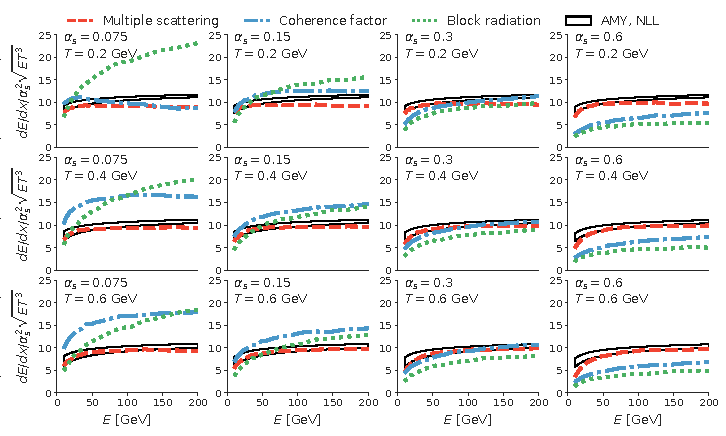
\includegraphics[width=\textwidth]{Eloss_infinite.pdf}
\caption{Energy loss per unit path lengh $dE/dx$ as a function of energy $E$, temperature $T$ and coupling constant $\alpha_s$. Each column corresponds to $\alpha_s = 0.075, 0.15, 0.3$, and $0.6$ (from left to right). Each column corresponds to $T = 0.2, 0.4$, and $0.6$ GeV (from top to bottom). $dE/dx$ is divided by the expected scaling $\alpha_s^2 \sqrt{ET^3}$. The calculations from ``Modified rescattering", ``Coherence factor", and ``Block radiation" approaches are the red-dashed lines, blue-dash-dotted lines, and green-dotted lines respectively. The AMY NLL results are denoted as black boxes.}
\label{fig:eloss-inf}
\end{figure*}

\section{Major results}
In this section, we compare the calculations of the three different implementations described in Section \ref{section:MC} to the theoretical limits quoted and described in Section \ref{section:Theo}. 

In Figure \ref{fig:eloss-inf}. We showed the calculation of energy loss per unit path length $dE/dx$ of a quark in an ``infinitely large" medium. 
Technically, we do a time evolution long enough so that any finite medium effect have faded away and then measure $dE/dx$.
The results presented are further divided by the anticipated scaling behavior $dE/dx \propto \alpha_s^2 \sqrt{ET^3}$.
For each column, we double the $\alpha_s$ value and for each row, temperature is increased by $0.2$ GeV. 
Within each subplot, the parton energy is varied from $10$ GeV to $200$ GeV.
Different Monte Carlo calculations are shown in colored lines, AMY NLL results are shown as black boxes. 
It is found that the ``Modified rescattering" approach (red-dashed lines) very well reproduces the energy, temperature, and coupling constant dependence of AMY NLL energy loss for relatively a high energy parton $E>20$ GeV.
At smaller energies, the simulated results decreases faster than the semi-analytic results.
For the ``Coherence factor" approach (blue-dash-dotted lines), although it does not include multiple rescatterings of the gluon. The energy dependence and temperature dependence are similar to the theoretical limits; however, it systematically deviates from the theory calculation for different coupling constant.
For the ``Blocking radiation" approaches, this $\alpha_s$-dependence deviation are even bigger, since we have seen in the previous section that suppression introduced by blocking other inelastic collisions within the formation of the current inelastic collision does not result in the correct power of $\alpha_s$ in the suppressed spectra.

Second we tested the path-length $L$ dependence of the energy loss $\Delta E$ of a quark with $E = 200$ GeV in a finite medium.
The comparison is showed in Figure \ref{fig:eloss-ldep}.
Again, each columns and each rows use different coupling constants and temperatures respectively and within each subplots the path length is varied up to a few times of $L_c^0$.
Here $L_c^0 = \sqrt{E/\hat{q}_0}$ is an estimate of the critical path length below which the non-linear $L$-dependence of $\Delta E$ should be prominent.


\begin{figure*}
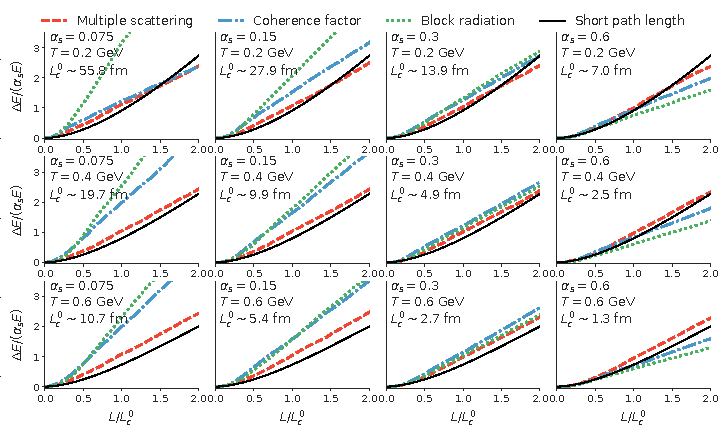
\includegraphics[width=\textwidth]{Eloss_Ldep.pdf}
\caption{Energy loss $\Delta E$ as a function of path length $L$, temperature $T$ and coupling constant $\alpha_s$. Each column corresponds to $\alpha_s = 0.075, 0.15, 0.3$, and $0.6$ (from left to right). Each column corresponds to $T = 0.2, 0.4$, and $0.6$ GeV (from top to bottom). $\Delta E$ is scaled by $\alpha_s E$ and $L$ is scaled by an estimated critical path length $L_c^0 = \sqrt{E/\hat{q}_0}$, $\hat{q}_0\sim 4\pi C_A\alpha_s^2 \times 1.28 T^3$. The calculations from ``Modified rescattering", ``Coherence factor", and ``Block radiation" approaches are the red-dashed lines, blue-dash-dotted lines, and green-dotted lines respectively. The analytic results for thin medium are denoted as black solid lines.}
\label{fig:eloss-ldep}
\end{figure*}

\section{Running coupling effect and expanding medium}
Before applying this new implementation to describe energetic parton transport in heavy ion collisions, there are still two more issues we need to study and address.
The first one is the study of LPM effect in an expanding medium. 
The QGP produced in colliders only exists for a short amount of time and it undergoes violent expansion, i.e, the medium temperature may have notably changed within the formation time.
Since the gluon receives coherent contributions during this time, one may expect a difference between the following two scenario:
\begin{itemize}
\item[1.] A direct calculation, where the total energy loss will be a functional of the temperature and fluid velocity space-time profile.$ \Delta E\left[ T(x), u^\mu(x) \right]$.
\item[2.] Using energy loss rate obtained in static medium set-up at different temperatures,
\begin{eqnarray}
\Delta E = \int \frac{dE}{dx}\left(T(x), u^\mu(x)\right) dx.
\end{eqnarray} 
\end{itemize} 
Although scenario 1 is closer to the realistic situation, we would like to see how big an effect the approximation 2 is for the case of heavy-ion collisions.
The ``Modified rescattering" approach allows us to study this since the gluon rescatterings are preformed at different space-time during the evolution.

The second to address is the running coupling constant. We follow the prescription described in []. For each gluon elastic rescatterings, we evaluate $\alpha_s$ at the momentum transfer of $t$-channel.




\section{Summary}
Moreover, one often implements the formula calculated for a static medium with a constant temperature, but the realistic medium in a heavy-ion collision undergoes fast expansion where temperature changes significantly within a time scale comparable to the LPM effect.
In this work, we studied three different Monte-Carlo implementations and systematically compare them to the semi-analytic theoretical limits.
We showed that by fine-tuning the parameters of one of the methods, the theoretical calculations are well reproduced at different coupling constants, parton energies, temperatures and path-lengths and this method generalizes to expanding medium. 
By showing that a Monte-Carlo implementation reduces to known theoretical calculation, a more meaning full theory-to-data comparison can be performed where the Monte-Carlo model works as a bridge between certain theory and experimental measurements.



\begin{acknowledgments}
SAB and WK  are supported by the U.S. Department of Energy Grant no. DE-FG02-05ER41367. WK is also supported by NSF grant OAC-1550225.
\end{acknowledgments}

\begin{appendices}
\end{appendices}
\bibliography{mclpm} 
\end{document}